% Source: PDF pages 14--20 (top).
\section{Constructions of combinatorial classes}
The idea is to build complicated classes from simple ones and translate these constructions into generating functions.

\subsection{Two basic classes}
\begin{enumerate}
\item The \textit{atomic class} $\mathcal Z=\{\bullet\}$ has a single object of size $1$. Its generating function is $z$.
\item The \textit{neutral class} $\mathcal E=\{\varepsilon\}$ has a single object of size $0$. Its generating function is $1$.
\end{enumerate}

\subsection{Sum}
\begin{definition}
Let $(A,|\cdot|_A)$ and $(B,|\cdot|_B)$ be combinatorial classes. The \textit{sum} $C=A+B$ is the class whose objects are the disjoint union of the objects in $A$ and $B$, with size
\[
|\sigma|_C=\begin{cases}|\sigma|_A,&\sigma\in A,\\|\sigma|_B,&\sigma\in B.\end{cases}
\]
\end{definition}
\begin{example}
If $\mathcal Z$ is the atomic class, then $\mathcal Z+\mathcal Z$ consists of two distinct atoms of size $1$.
\end{example}
\begin{lemma}
If $C=A+B$, then $C(z)=A(z)+B(z)$.
\end{lemma}
\begin{proof}
An object of size $n$ in $C$ is an object of size $n$ in $A$ or in $B$. Because the union is disjoint, $c_n=a_n+b_n$. Thus
\begin{align*}
C(z)&=\sum_{n\ge0}c_nz^n
=\sum_{n\ge0}(a_n+b_n)z^n\\
&=\sum_{n\ge0}a_nz^n+\sum_{n\ge0}b_nz^n=A(z)+B(z).
\end{align*}
\end{proof}

\subsection{Product and powers}
\begin{definition}
The \textit{product} $C=A\times B$ is the class of all pairs
\[
\{(\alpha,\beta):\alpha\in A,\ \beta\in B\},
\qquad |(\alpha,\beta)|_C=|\alpha|_A+|\beta|_B.
\]
\end{definition}
\begin{lemma}
If $C=A\times B$, then $C(z)=A(z)B(z)$.
\end{lemma}
\begin{proof}
\begin{align*}
C(z)&=\sum_{(\alpha,\beta)\in C}z^{|(\alpha,\beta)|}
=\sum_{(\alpha,\beta)\in C}z^{|\alpha|_A+|\beta|_B}\\
&=\left(\sum_{\alpha\in A}z^{|\alpha|_A}\right)
\left(\sum_{\beta\in B}z^{|\beta|_B}\right)=A(z)B(z).
\end{align*}
\end{proof}
For any positive integer $k$, the \textit{power}
\[
A^k=\underbrace{A\times A\times\cdots\times A}_{k\text{ times}}
=\{(\alpha_1,\ldots,\alpha_k):\alpha_i\in A\}
\]
has generating function $A(z)^k$.

\subsection{Sequences}
\begin{definition}
Let $A$ be a combinatorial class with no objects of size $0$. Its \textit{sequence class} is
\[
\operatorname{SEQ}(A)=\mathcal E+A+A^2+\cdots
=\bigcup_{k\ge0}\{(\alpha_1,\ldots,\alpha_k):\alpha_i\in A\}.
\]
\end{definition}
If $A$ had an object of size $0$, then $\operatorname{SEQ}(A)$ would have infinitely many objects of size $0$.
\begin{lemma}
If $C=\operatorname{SEQ}(A)$, then
\[
C(z)=1+A(z)+A(z)^2+\cdots=\frac1{1-A(z)}.
\]
\end{lemma}
\begin{example}
Let $B$ be the class of binary strings. Taking the atoms $\mathcal Z_0=\{0\}$ and $\mathcal Z_1=\{1\}$,
\[
B=\operatorname{SEQ}(\mathcal Z_0+\mathcal Z_1),
\qquad B(z)=\frac1{1-(z+z)}=\frac1{1-2z}.
\]
\end{example}
\begin{definition}
An \textit{integer composition} of size $n$ is a tuple of positive integers whose sum is $n$.
\end{definition}
\begin{example}
The compositions of size $3$ are $(3)$, $(2,1)$, $(1,2)$, and $(1,1,1)$, corresponding to
$3$, $2+1$, $1+2$, and $1+1+1$.
If order does not matter, the corresponding object is a partition.

Let $P$ be the class of positive integers, with $|n|=n$, and let $C$ be the class of compositions. Then
\[
C=\operatorname{SEQ}(P),\qquad
P=\mathcal Z\times\operatorname{SEQ}(\mathcal Z).
\]
The initial atom ensures that the integer is positive, because $\operatorname{SEQ}(\mathcal Z)$ includes the empty object. Thus
\[
P(z)=\frac z{1-z},\qquad
C(z)=\frac1{1-\frac z{1-z}}=\frac{1-z}{1-2z}.
\]
For $n\ge1$,
\begin{align*}
[z^n]C(z)&=[z^n]\frac{1-z}{1-2z}\\
&=[z^n]\left(\frac1{1-2z}-\frac z{1-2z}\right)\\
&=2^n-[z^{n-1}]\frac1{1-2z}\\
&=2^n-2^{n-1}=2^{n-1}.
\end{align*}
The restriction $n\ge1$ is necessary; the empty composition gives $[z^0]C(z)=1$.
\end{example}

Restricted sequence constructions give
\begin{align*}
\operatorname{SEQ}_{\le r}(A)&=\mathcal E+A+\cdots+A^r,
& C(z)&=\frac{1-A(z)^{r+1}}{1-A(z)},\\
\operatorname{SEQ}_{\ge r}(A)&=A^r+A^{r+1}+\cdots,
& C(z)&=\frac{A(z)^r}{1-A(z)},\\
\operatorname{SEQ}_{\mathrm{even}}(A)&=\mathcal E+A^2+A^4+\cdots,
& C(z)&=\frac1{1-A(z)^2}.
\end{align*}

\subsection{Iterative and recursive constructions}
There are two types of constructions: \textit{iterative} and \textit{recursive}.
\begin{example}
A rooted planar binary tree is either empty or has a root vertex followed by a possibly empty left subtree and a possibly empty right subtree. In particular, a single root vertex is allowed.
\begin{center}
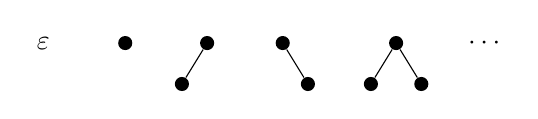
\begin{tikzpicture}[x=.8cm,y=.8cm,v/.style={circle,fill,inner sep=1.8pt}]
\node at (0,0) {$\varepsilon$};
\node[v] at (1.3,0) {};
\node[v] (a) at (2.6,0) {}; \node[v] (b) at (2.2,-.65) {}; \draw (a)--(b);
\node[v] (c) at (3.8,0) {}; \node[v] (d) at (4.2,-.65) {}; \draw (c)--(d);
\node[v] (e) at (5.6,0) {}; \node[v] (f) at (5.2,-.65) {}; \node[v] (g) at (6,-.65) {}; \draw (f)--(e)--(g);
\node at (7,0) {$\cdots$};
\end{tikzpicture}
\end{center}

If $B$ is the class of these trees, then
\[
B=\mathcal E+\mathcal Z\times B\times B.
\]
The four components mean: empty tree, root, left subtree, and right subtree. Therefore
\[
B(z)=1+zB(z)^2,
\qquad zB(z)^2-B(z)+1=0,
\]
so $B(z)$ is one of the two solutions
\[
\frac{1\pm\sqrt{1-4z}}{2z}.
\]
The plus sign gives
\[
\frac{1+\sqrt{1-4z}}{2z}
=\frac{2-2z+\cdots}{2z}=\frac1z-1+\cdots,
\]
which is not a formal power series.
% The source's wording omits the empty-tree case in its first sentence;
% its examples and recursive specification explicitly include it.
\end{example}
Therefore the binary-tree generating function is
\[
B(z)=\frac{1-\sqrt{1-4z}}{2z}
=1+z+2z^2+\cdots
=\sum_{n\ge0}\frac1{n+1}\binom{2n}{n}z^n.
\]
This counts the possible binary trees of a given size; the source also notes its relevance to estimating the number of bits needed to encode a binary tree.
